\section{需求分析与调研}

\subsection{需求分析}

根据题目描述,我们需要实现一个“更加智能的 Flash 文件系统”。

Flash介质因本身的擦除特性,给上层文件系统带来与普通磁盘、内存文件系统不同的数据管理模式。
同时,Flash的写入放大、寿命以及后期稳定性下降等问题也给文件系统的设计带来的一定的挑战。
传统的Flash文件系统并没有很好地解决这些稳定性相关问题。
这里希望寻找一种更智能、更合适的Flash文件系统设计,来更好地平衡Flash的性能与稳定性。
可以思考的方向包括但不限于:数据压缩算法(可以是自适应的压缩算法),检错、纠错、纠删码(可以是联合信源信道编码),数据块选择、擦除策略,Cache机制。

结合赛题内容,我们需要完成的文件系统需要具备以下特性:

\begin{itemize}
  \item {\bf{适合 Flash 介质}}:文件系统需要能够适应并缓解 Flash 的写入放大、寿命、后期稳定性等诸多 Flash 存储介质特有的问题
  \item {\bf{更智能}}:文件系统需要使用多种策略,在软件算法层面平衡性能与寿命
\end{itemize}

\subsubsection{背景调研}

\subsubsubsection{往年实现分析}

本题在去年已经有队伍完成,他们的仓库在 \url{https://gitlab.eduxiji.net/why/project788067-124640}。
在选题之时,我们对其进行了调研。

他们队伍完成了一个基于 UBIFS 的适用于裸 Flash 设备的 YOUBIFS 文件系统,从以下几个方面对其进行了优化:

\begin{itemize}
  \item {\bf{数据压缩模块}}:使用了预压缩和自适应压缩结合的方法,均衡压缩比和写入速度
  \item {\bf{纠错编码模块}}:实现自适应生命周期、CRC+RAID5两种纠错方案
  \item {\bf{Cache 机制}}:添加读写缓冲
  \item {\bf{冷热数据识别}}:使用了冷热识别的纠错以提高 I/O 速度
\end{itemize}

\begin{figure}[htbp]
  \centering
  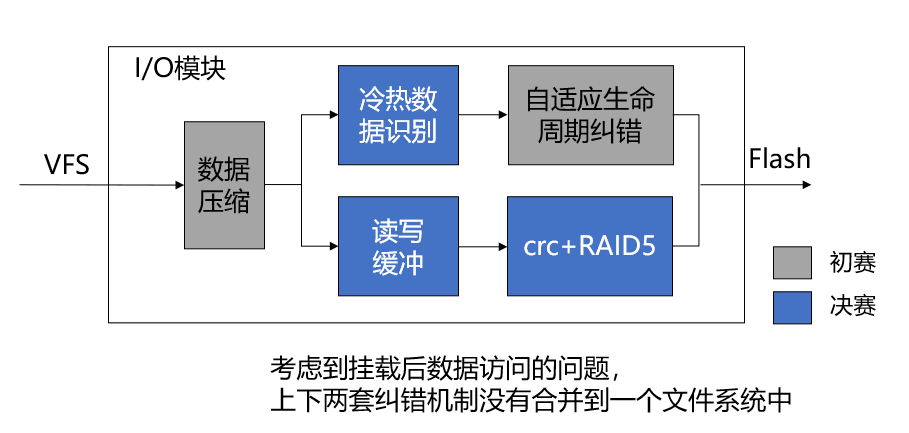
\includegraphics[width=0.7\textwidth]{fig/YOUBIFS项目框图.png}
  \caption{YOUBIFS 系统架构}
  \label{youbifs}
\end{figure}

YOUBIFS 的系统架构如图 \ref{youbifs} 所示。
看起来 YOUBIFS 的实现已经非常满足题目的需求,能够很好地回答题目中提出的几个问题。
但是我们发现,YOUBIFS 的系统实现也存在一些不足之处:

\begin{itemize}
  \item {\bf{Nor Flash 应用场景}}
    
  YOUBIFS 的实现中,文件系统的实现是针对于 Nor Flash 的。
  Nor Flash 在实现上与 Nand Flash 有很大的不同,因此 YOUBIFS 的实现并不能直接应用于 Nand Flash 上,应用场景受到了限制。
  
  同时,Nor Flash 一般用于嵌入式设备,而 Nand Flash 一般用于移动设备或高性能设备,因此 YOUBIFS 的实现也不能直接应用于移动设备或固态硬盘上。
  YOUBIFS 针对于 Nor Flash 的多种写入情况做了优化,但是由于 Nor Flash 的寿命、速度、稳定性等特性,其并不适合在写入负载较高的情况下工作。

  Nor Flash 的寿命一般在 10 万次左右,而 Nand Flash 的寿命一般在 100 万次左右,因此 Nor Flash 广泛用于 BIOS 存储、固件存储等写入负载较低的场景。
  在这些应用场景下,由于存储的数据都是非常重要的系统关键数据,如 Bootloader、系统固件等,因此对于数据的稳定性要求非常高。
  如果系统软件直接在 Nor Flash 上频繁读写,很可能会导致 Nor Flash 的寿命过早耗尽,从而导致系统无法正常启动,造成非常严重的后果。

  因此,YOUFIBS 的实现并不能直接应用于移动设备或固态硬盘上,也不能直接应用于写入负载较高的场景。
  这与 YOUBIFS 的各种优化策略相矛盾,因此我们需要重新设计一个适用于 Nand Flash 的文件系统。

  \item {\bf{“智能”,但是还不够智能}}

  YOUBIFS 的实现中,使用了多种策略来平衡性能与寿命,但是这些策略都是相对固定的,只是能够根据不同的情况进行策略切换。
  其中能够体现“智能”的实现有:

  \begin{enumerate}
    \item 通过判断文件名的方式来判断使用的压缩算法和参数,即压缩算法和等级的自适应
    \item 通过检查压缩效果是否合适来判断是否继续压缩,压缩效果不好可能其数据本身就是压缩文件,则再次不压缩
    \item 利用文件系统中的局部性,判别冷热数据文件
    \item 在 Flash 后期容易产生错误的时候转用纠错能力更强的算法
  \end{enumerate}

\end{itemize}